\section{Thiết lập cụm Pseudo-distributed}
\label{sec:pseudo-distributed}

% Rubric: "Successfully install Hadoop (NameNode, DataNode)" = 1.0 pt
% Rubric: "Detailed report (setup, step-by-step, errors)" = 1.0 pt
% Cài đặt trực tiếp trên OS, KHÔNG dùng image có sẵn (FAQ Q3)

Phần này trình bày chi tiết quá trình thiết lập cụm Hadoop ở chế độ Pseudo-distributed (giả phân tán), trong đó mỗi tiến trình Hadoop (NameNode, DataNode, ResourceManager, NodeManager) chạy như một tiến trình Java độc lập trên cùng một máy tính. Việc cài đặt được thực hiện trực tiếp trên hệ điều hành (native), không sử dụng Docker image có sẵn, tuân thủ yêu cầu của bài thực hành \cite{white2012hadoop}.

\subsection{Phương thức cài đặt}

\begin{table}[H]
\centering
\caption{Thông tin môi trường cài đặt.}
\label{tab:env-info}
\begin{tabular}{ll}
\toprule
\textbf{Thành phần} & \textbf{Chi tiết} \\
\midrule
Hệ điều hành & Arch Linux (kernel 6.19.10) \\
Shell mặc định & fish \\
Phương thức cài đặt & Native (trực tiếp trên OS) \\
Phiên bản Java & OpenJDK 8 \\
Phiên bản Hadoop & 3.4.3 \\
Thư mục cài đặt & \texttt{/opt/hadoop} \\
\bottomrule
\end{tabular}
\end{table}

% TODO: [USER] Cập nhật kernel version cho chính xác

\subsection{Quá trình cài đặt}

\subsubsection{Cài đặt Java}

Hadoop yêu cầu Java 8 hoặc Java 11. Trên Arch Linux, OpenJDK được cài đặt thông qua trình quản lý gói \texttt{pacman}:

\begin{lstlisting}[language=bash, numbers=none]
sudo pacman -S jdk8-openjdk
\end{lstlisting}

Xác minh phiên bản Java đã cài đặt thành công:

\begin{lstlisting}[language=bash, numbers=none]
java -version
\end{lstlisting}

\begin{figure}[H]
    \centering
    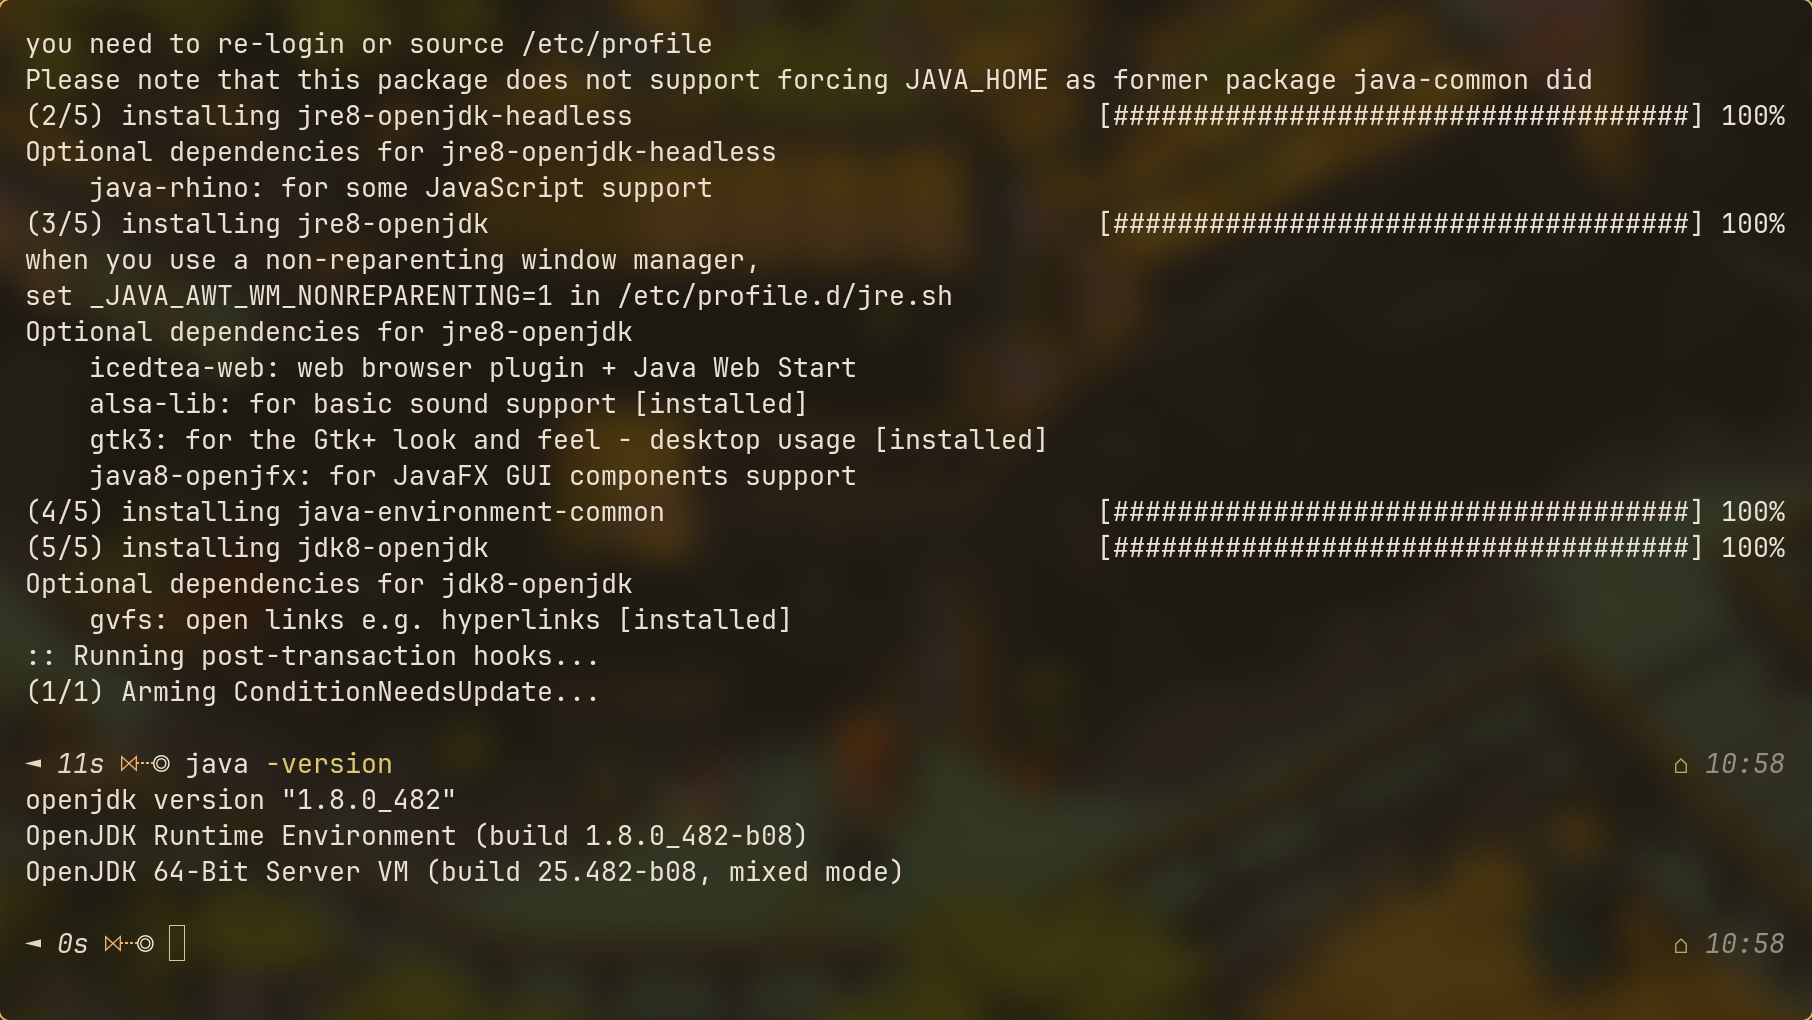
\includegraphics[width=0.8\textwidth]{images/pseudo-1.png}
    \caption{Xác minh phiên bản Java đã cài đặt.}
    \label{fig:pseudo-java}
\end{figure}

\subsubsection{Cài đặt và cấu hình SSH}

Hadoop sử dụng SSH để quản lý các tiến trình daemon ngay cả trong chế độ pseudo-distributed. Gói \texttt{openssh} được cài đặt từ repo chính thức, còn \texttt{pdsh} (Parallel Distributed Shell) không có trong repo của Arch nên phải cài từ AUR:

\begin{lstlisting}[language=bash, numbers=none]
# openssh co san trong repo chinh thuc
sudo pacman -S openssh
sudo systemctl enable --now sshd

# pdsh chi co tren AUR
paru -S pdsh
\end{lstlisting}

Tiếp theo, thiết lập đăng nhập SSH không mật khẩu (passphraseless SSH) — điều kiện bắt buộc để các script khởi động của Hadoop hoạt động:

\begin{lstlisting}[language=bash, numbers=none]
ssh-keygen -t rsa -P '' -f ~/.ssh/id_rsa
cat ~/.ssh/id_rsa.pub >> ~/.ssh/authorized_keys
chmod 0600 ~/.ssh/authorized_keys
\end{lstlisting}

Kiểm tra kết nối:

\begin{lstlisting}[language=bash, numbers=none]
ssh localhost
\end{lstlisting}

\begin{figure}[H]
    \centering
    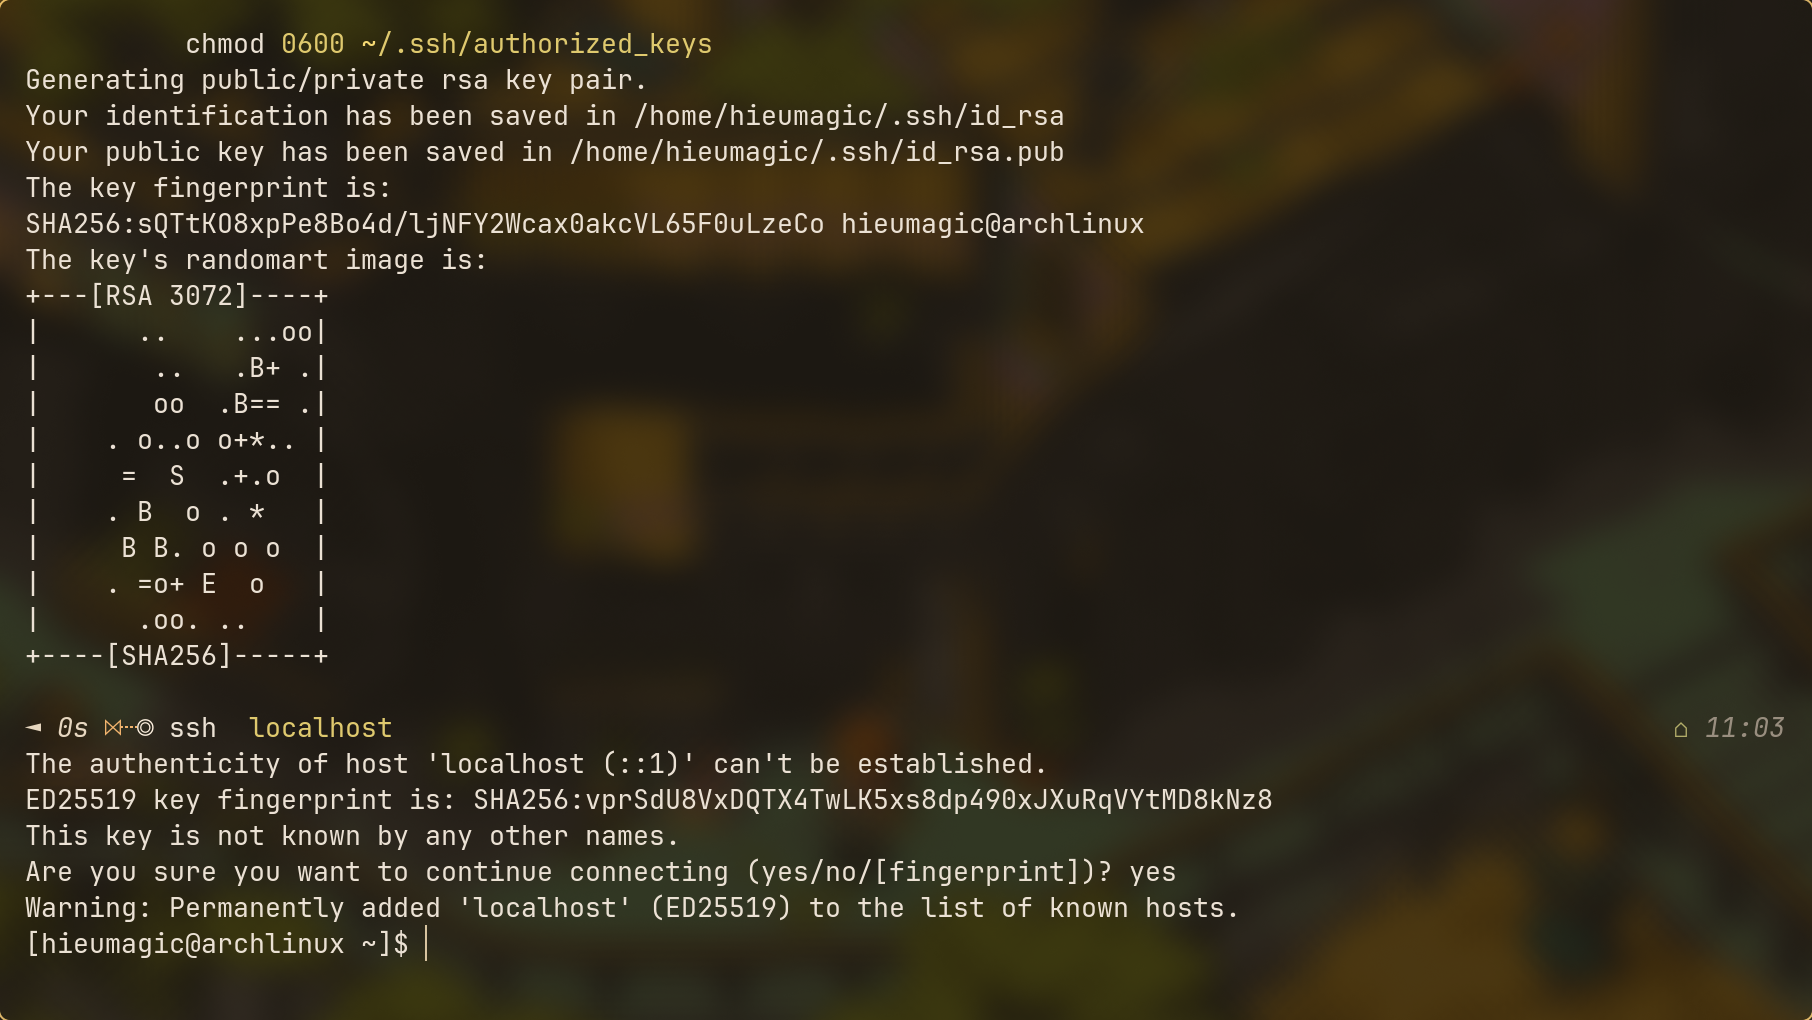
\includegraphics[width=0.8\textwidth]{images/pseudo-2.png}
    \caption{Xác minh kết nối SSH không mật khẩu tới localhost.}
    \label{fig:pseudo-ssh}
\end{figure}

\subsubsection{Tải và cài đặt Hadoop}

Bản phân phối Hadoop được tải trực tiếp từ Apache Mirror chính thức, giải nén và đặt tại thư mục \texttt{/opt/hadoop}:

\begin{lstlisting}[language=bash, numbers=none]
wget https://dlcdn.apache.org/hadoop/common/hadoop-3.4.3/hadoop-3.4.3.tar.gz
tar -xzf hadoop-3.4.3.tar.gz
sudo mv hadoop-3.4.3 /opt/hadoop
sudo chown -R $(whoami):$(whoami) /opt/hadoop
\end{lstlisting}

Do shell mặc định là \texttt{fish} (không tương thích cú pháp \texttt{export} của Bash), các biến môi trường được thiết lập trong tệp \texttt{\textasciitilde/.config/fish/config.fish}:

\begin{lstlisting}[language=bash, numbers=none, caption={Cấu hình biến môi trường trong fish shell.}]
set -x JAVA_HOME /usr/lib/jvm/java-8-openjdk
set -x HADOOP_HOME /opt/hadoop
set -x HADOOP_CONF_DIR $HADOOP_HOME/etc/hadoop
set -x HADOOP_MAPRED_HOME $HADOOP_HOME
set -x PATH $HADOOP_HOME/bin $HADOOP_HOME/sbin $PATH
set -x PDSH_RCMD_TYPE ssh
\end{lstlisting}

Biến \texttt{PDSH\_RCMD\_TYPE} được đặt thành \texttt{ssh} để \texttt{pdsh} sử dụng SSH thay vì \texttt{rsh} (mặc định), tránh lỗi kết nối khi khởi động daemon.

Ngoài ra, \texttt{JAVA\_HOME} cũng phải được khai báo trong tệp \texttt{hadoop-env.sh} vì các script Hadoop sử dụng Bash và không kế thừa biến môi trường từ fish:

\begin{lstlisting}[language=bash, numbers=none]
# Trong $HADOOP_HOME/etc/hadoop/hadoop-env.sh
export JAVA_HOME=/usr/lib/jvm/java-8-openjdk
\end{lstlisting}

Xác minh cài đặt thành công:

\begin{lstlisting}[language=bash, numbers=none]
hadoop version
\end{lstlisting}

\begin{figure}[H]
    \centering
    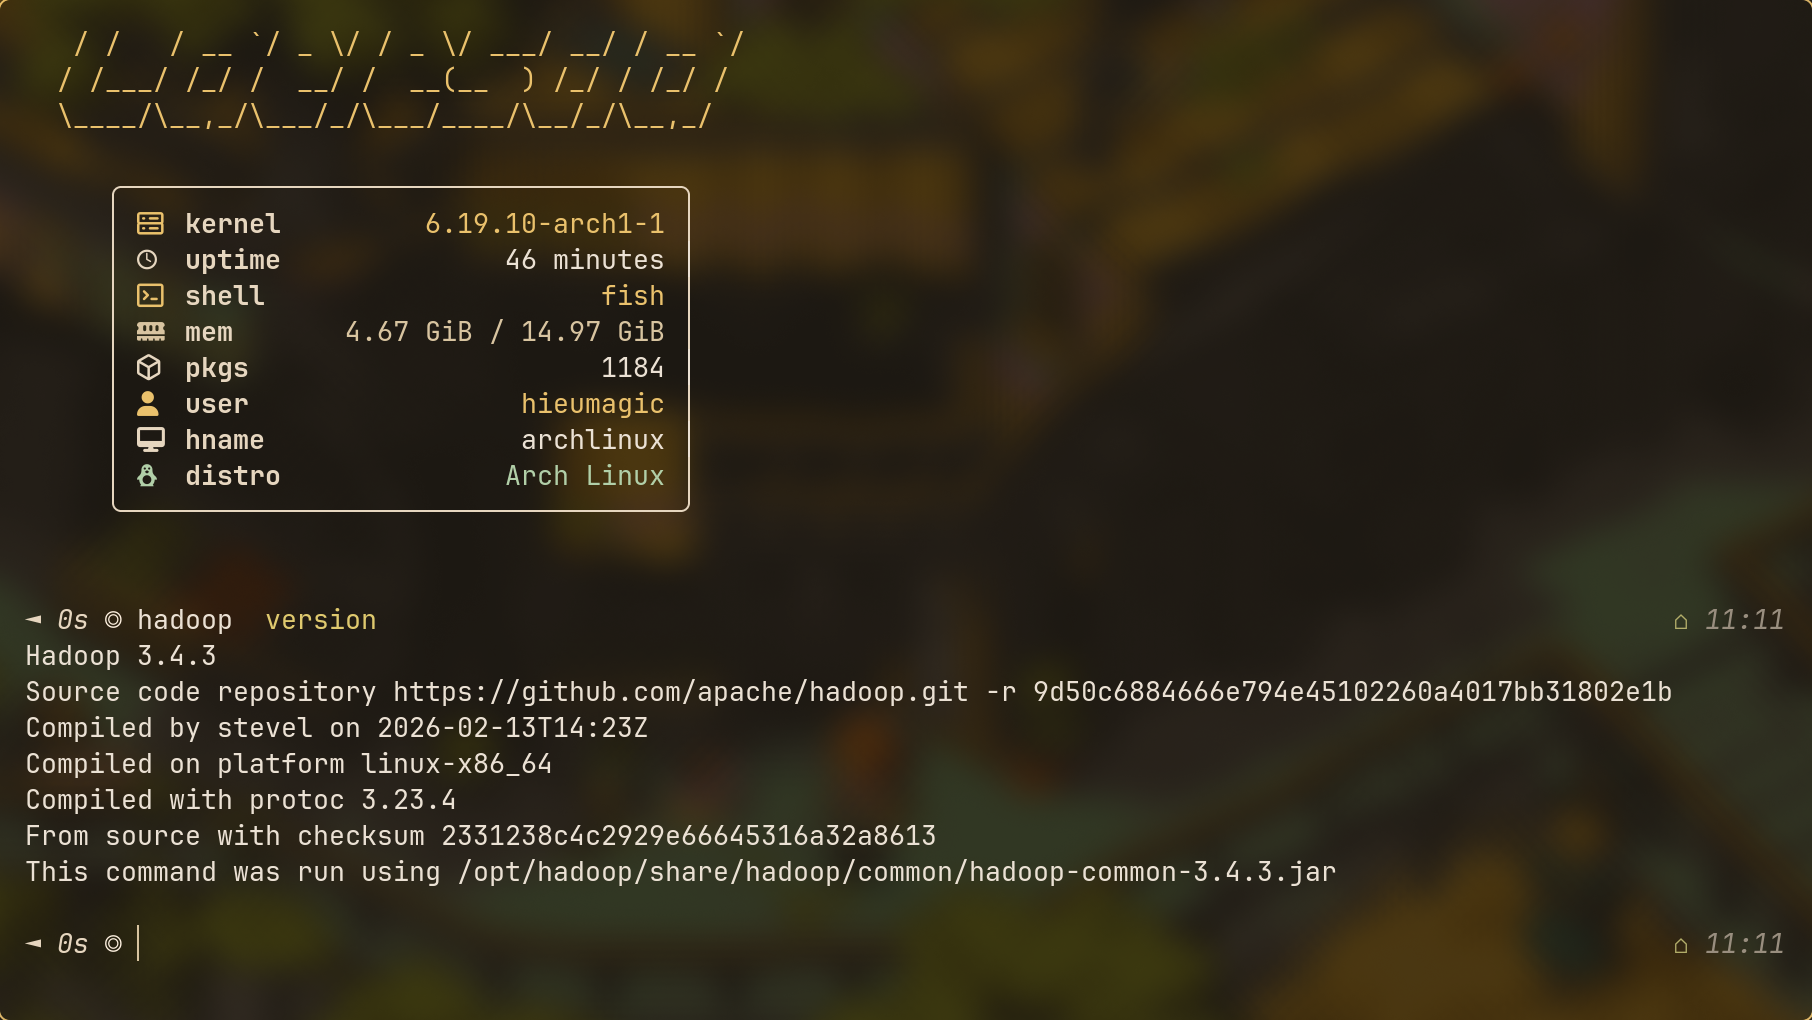
\includegraphics[width=0.8\textwidth]{images/pseudo-3.png}
    \caption{Xác minh phiên bản Hadoop đã cài đặt.}
    \label{fig:pseudo-hadoop-version}
\end{figure}

\subsubsection{Cấu hình các tệp XML}

Bốn tệp cấu hình chính trong thư mục \texttt{\$HADOOP\_HOME/etc/hadoop/} được chỉnh sửa theo hướng dẫn chính thức của Apache\footnote{\url{https://hadoop.apache.org/docs/stable/hadoop-project-dist/hadoop-common/SingleCluster.html}}:

\paragraph{core-site.xml} — Thiết lập địa chỉ hệ thống tệp mặc định:

\begin{lstlisting}[language=xml, numbers=none]
<configuration>
    <property>
        <name>fs.defaultFS</name>
        <value>hdfs://localhost:9000</value>
    </property>
</configuration>
\end{lstlisting}

\paragraph{hdfs-site.xml} — Đặt hệ số nhân bản bằng 1 (chỉ có một DataNode):

\begin{lstlisting}[language=xml, numbers=none]
<configuration>
    <property>
        <name>dfs.replication</name>
        <value>1</value>
    </property>
</configuration>
\end{lstlisting}

\paragraph{mapred-site.xml} — Chỉ định YARN làm framework thực thi MapReduce:

\begin{lstlisting}[language=xml, numbers=none]
<configuration>
    <property>
        <name>mapreduce.framework.name</name>
        <value>yarn</value>
    </property>
    <property>
        <name>mapreduce.application.classpath</name>
        <value>$HADOOP_MAPRED_HOME/share/hadoop/mapreduce/*:
               $HADOOP_MAPRED_HOME/share/hadoop/mapreduce/lib/*
        </value>
    </property>
</configuration>
\end{lstlisting}

\paragraph{yarn-site.xml} — Kích hoạt dịch vụ phụ trợ shuffle cho MapReduce:

\begin{lstlisting}[language=xml, numbers=none]
<configuration>
    <property>
        <name>yarn.nodemanager.aux-services</name>
        <value>mapreduce_shuffle</value>
    </property>
    <property>
        <name>yarn.nodemanager.env-whitelist</name>
        <value>JAVA_HOME,HADOOP_COMMON_HOME,HADOOP_HDFS_HOME,
               HADOOP_CONF_DIR,CLASSPATH_PREPEND_DISTCACHE,
               HADOOP_YARN_HOME,HADOOP_HOME,PATH,LANG,TZ,
               HADOOP_MAPRED_HOME</value>
    </property>
</configuration>
\end{lstlisting}

\begin{figure}[H]
    \centering
    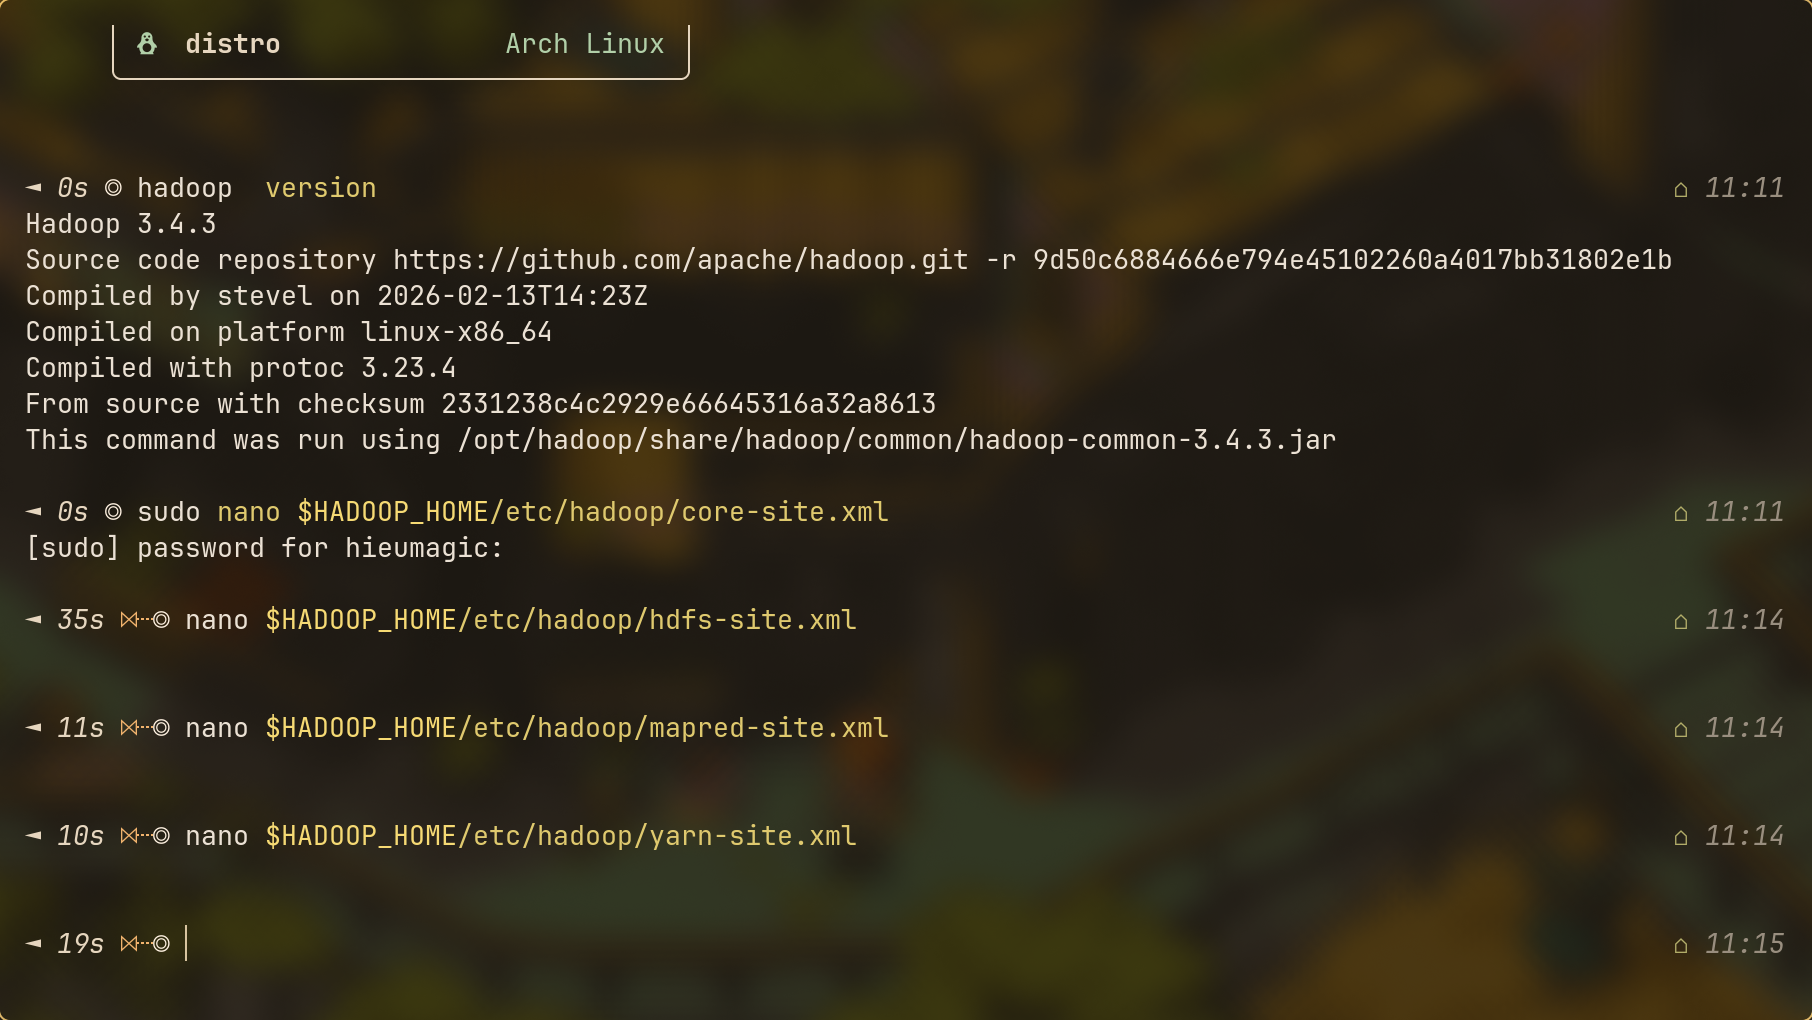
\includegraphics[width=0.8\textwidth]{images/pseudo-4.png}
    \caption{Cấu hình bốn tệp XML chính cho chế độ Pseudo-distributed.}
    \label{fig:pseudo-xml-config}
\end{figure}

\subsubsection{Định dạng NameNode và khởi động dịch vụ}

Trước khi khởi động lần đầu, hệ thống tệp HDFS cần được định dạng (format):

\begin{lstlisting}[language=bash, numbers=none]
hdfs namenode -format
\end{lstlisting}

\begin{figure}[H]
    \centering
    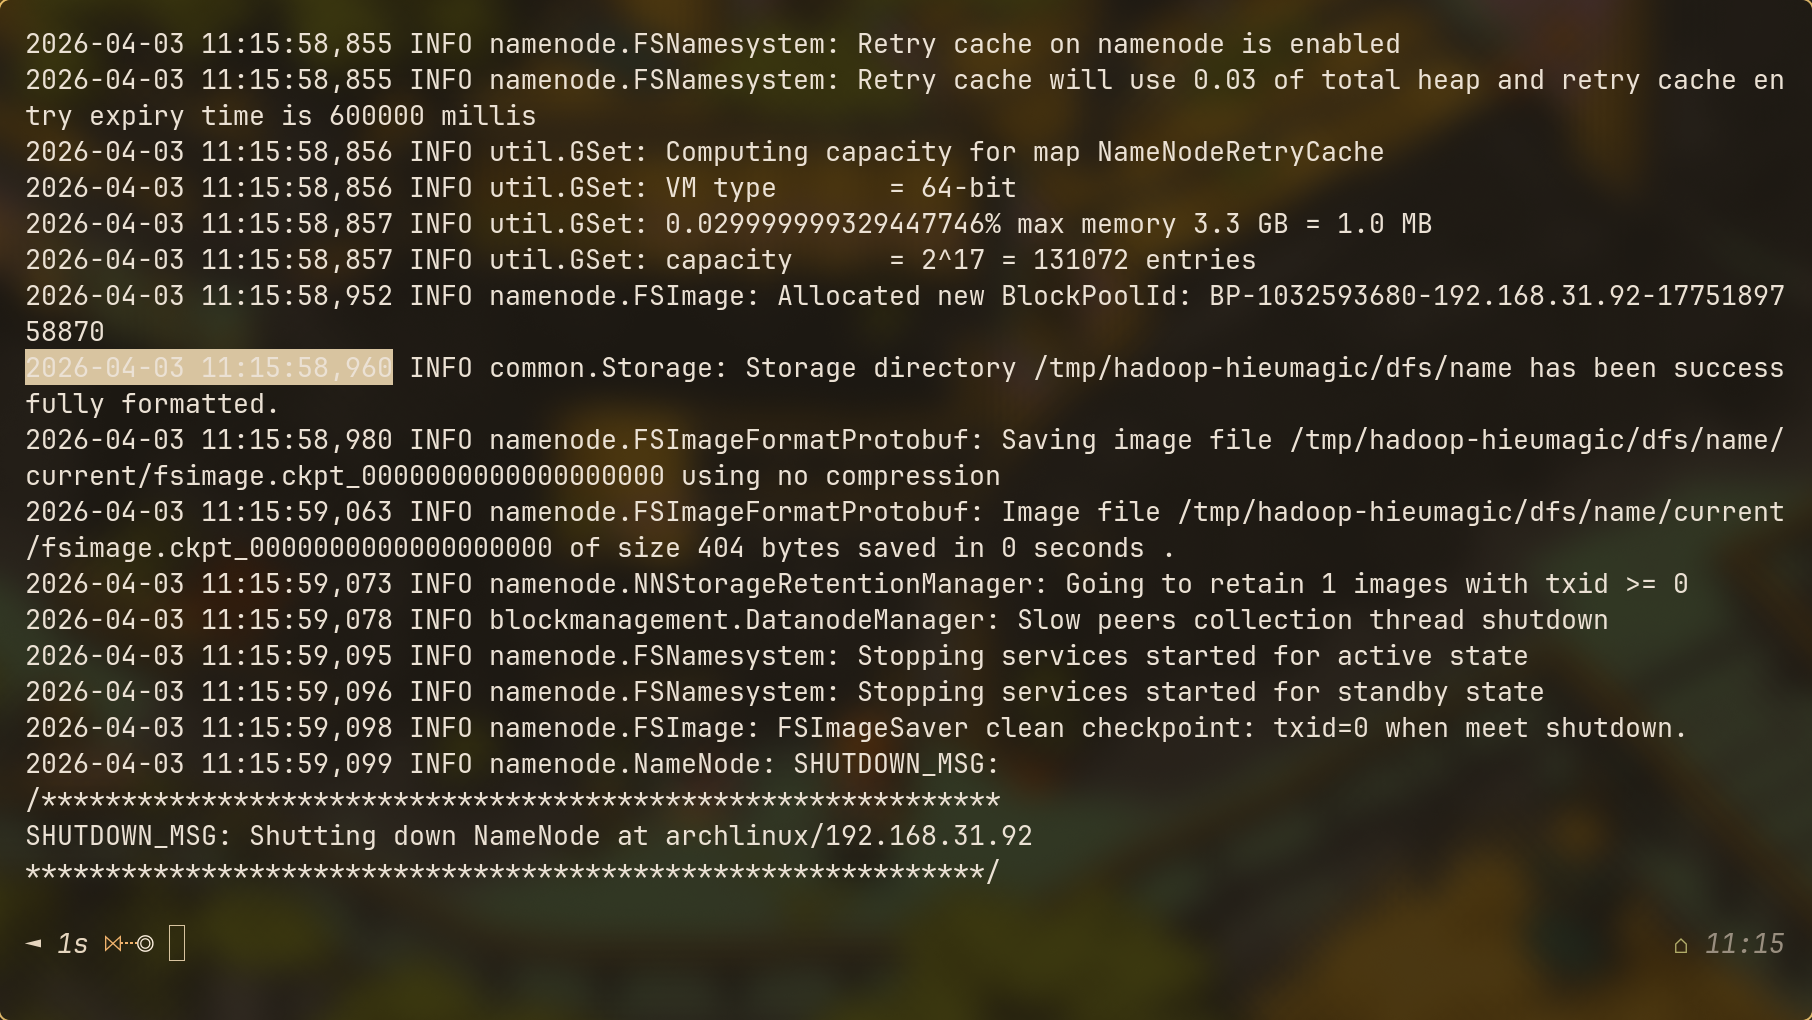
\includegraphics[width=0.8\textwidth]{images/pseudo-5.png}
    \caption{Định dạng hệ thống tệp HDFS lần đầu.}
    \label{fig:pseudo-format}
\end{figure}

Khởi động HDFS (NameNode + DataNode) và YARN (ResourceManager + NodeManager):

\begin{lstlisting}[language=bash, numbers=none]
start-dfs.sh
start-yarn.sh
\end{lstlisting}

\begin{figure}[H]
    \centering
    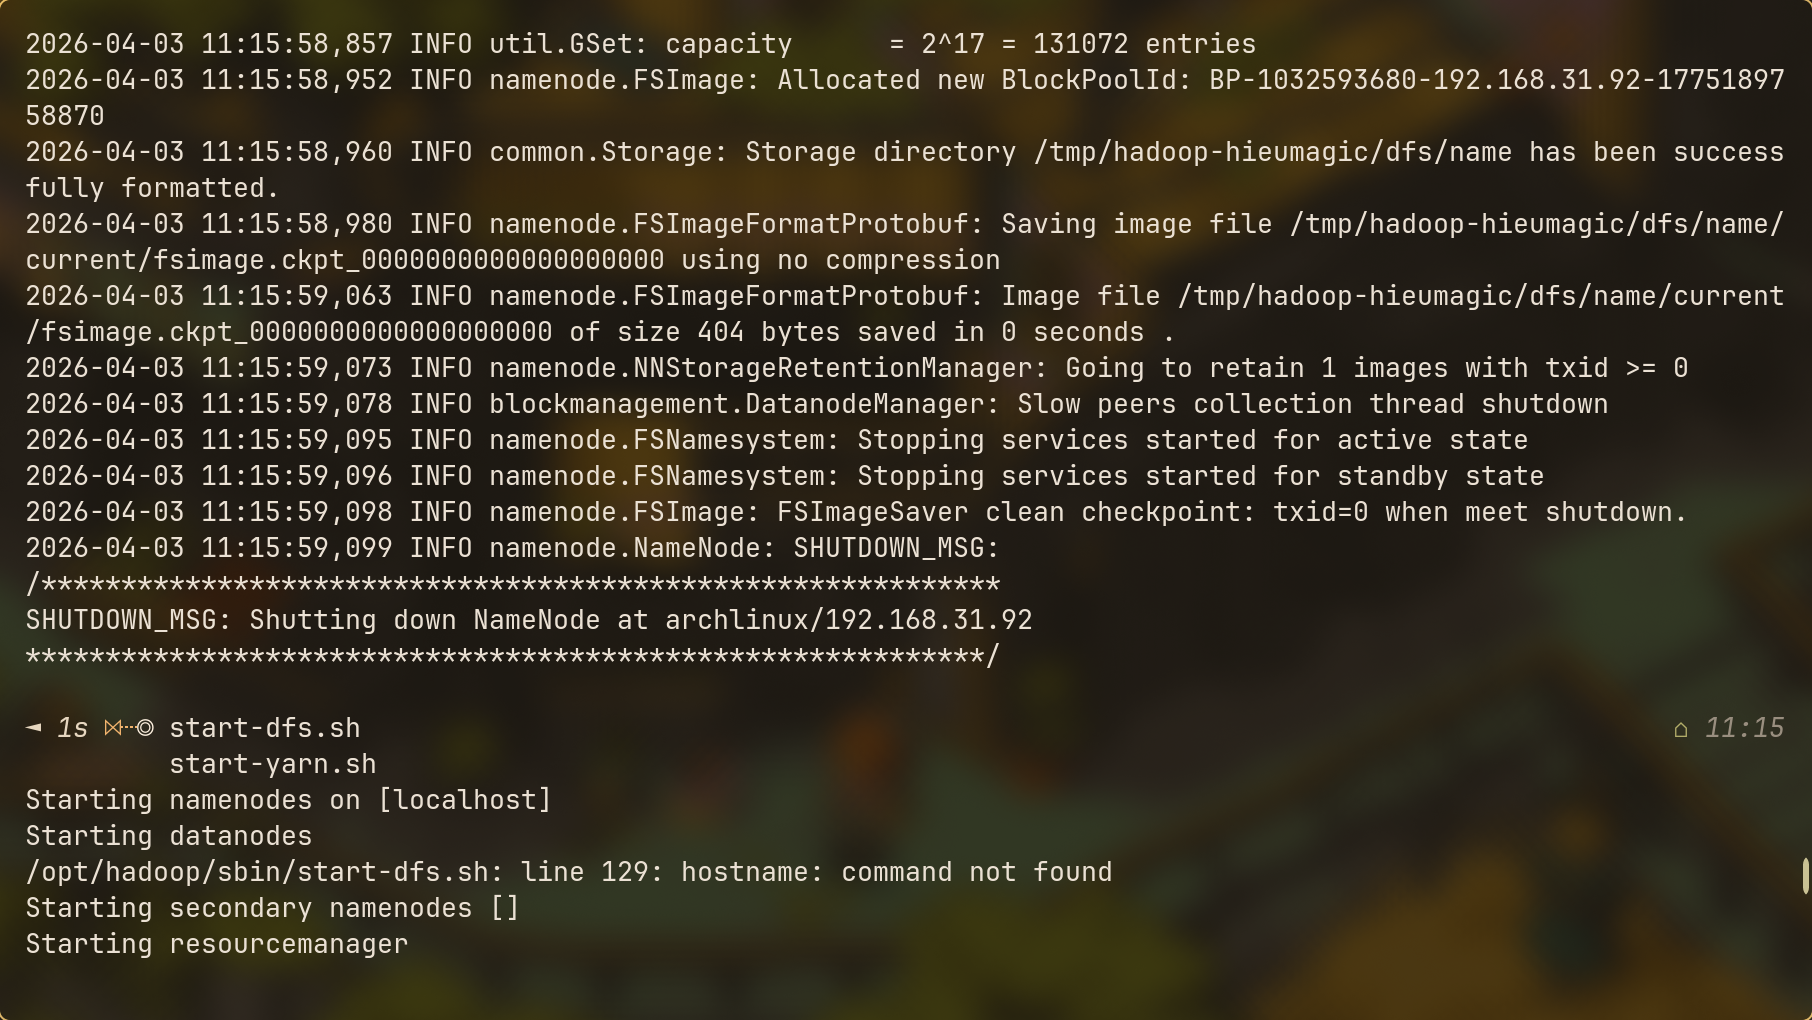
\includegraphics[width=0.8\textwidth]{images/pseudo-6.png}
    \caption{Khởi động các dịch vụ HDFS và YARN.}
    \label{fig:pseudo-start}
\end{figure}

\subsection{Xác minh hệ thống}

\subsubsection{Kiểm tra tiến trình với JPS}

Lệnh \texttt{jps} (Java Virtual Machine Process Status) xác nhận tất cả các daemon đang hoạt động:

\begin{lstlisting}[language=bash, numbers=none]
jps
\end{lstlisting}

Kết quả mong đợi phải hiển thị đủ 5 tiến trình: \texttt{NameNode}, \texttt{DataNode}, \texttt{SecondaryNameNode}, \texttt{ResourceManager} và \texttt{NodeManager}.

\begin{figure}[H]
    \centering
    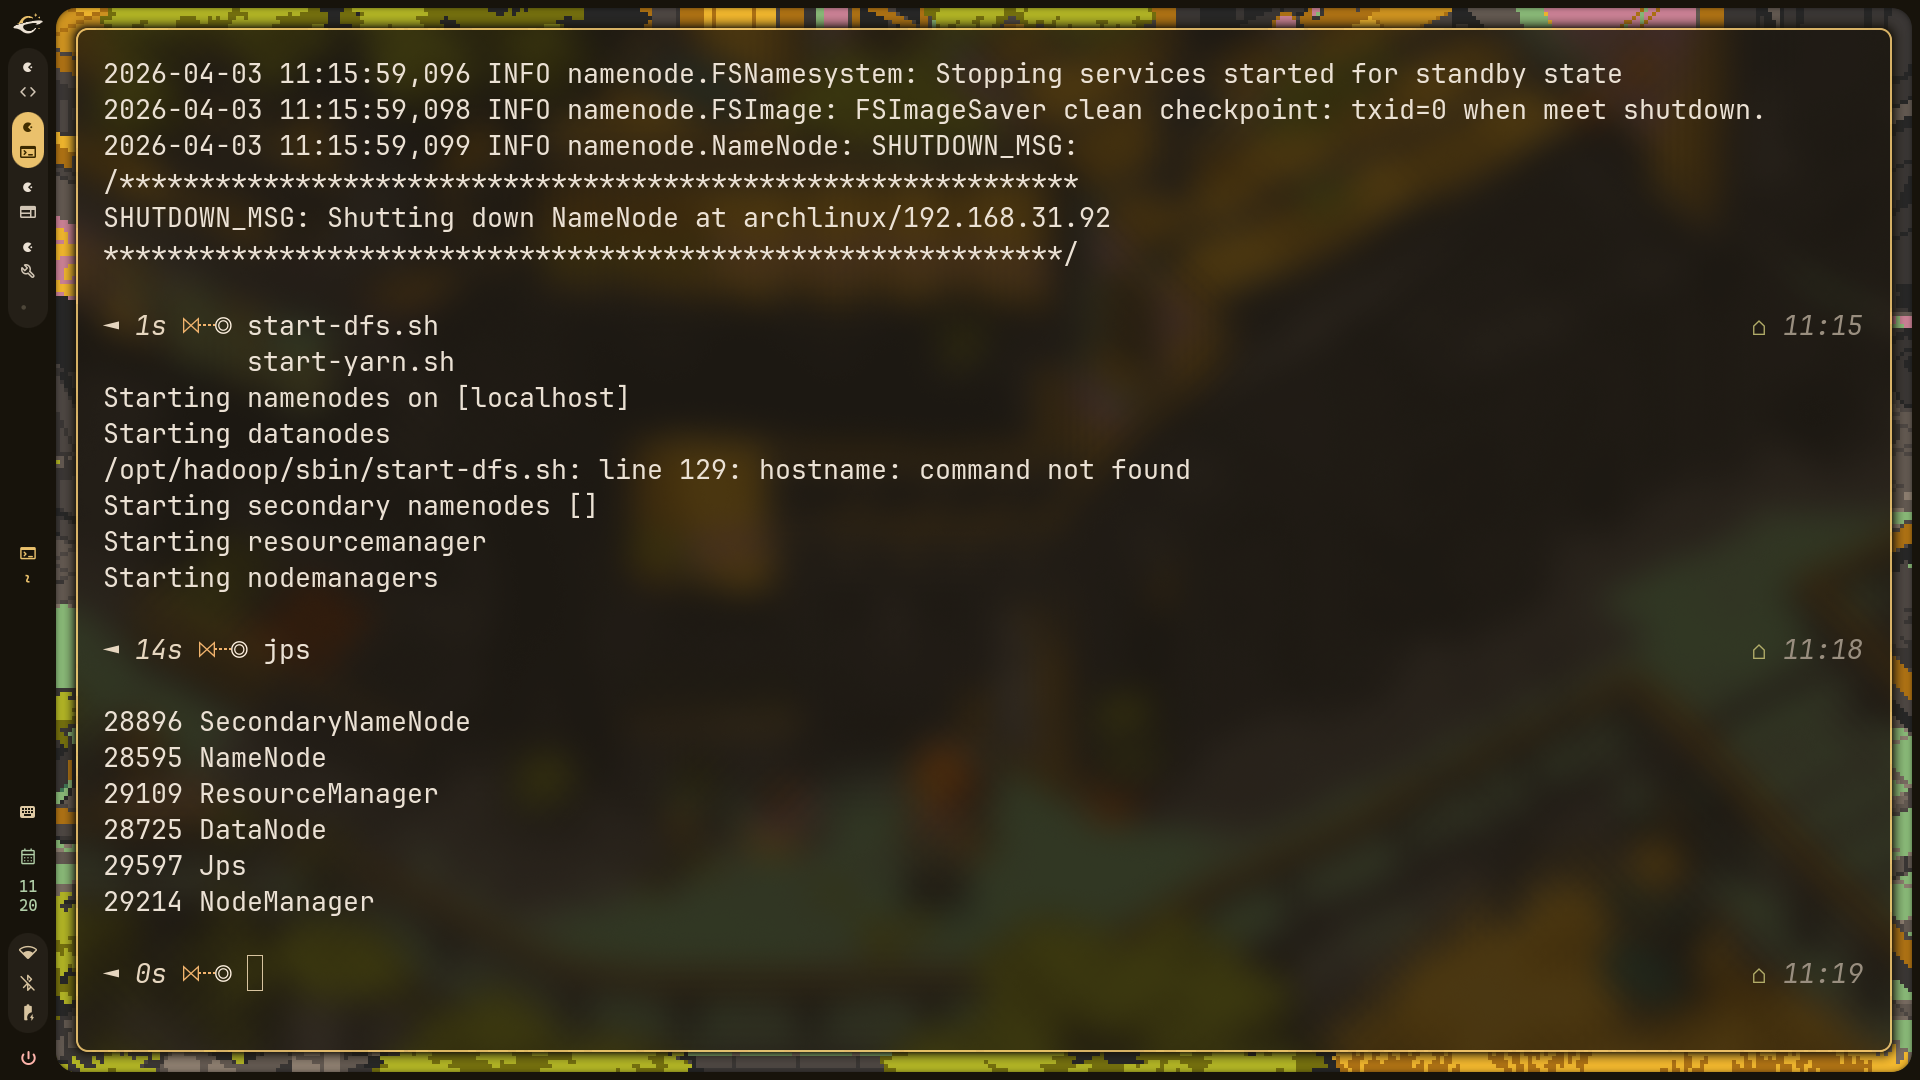
\includegraphics[width=0.6\textwidth]{images/pseudo-7.png}
    \caption{Danh sách tiến trình Hadoop đang hoạt động qua lệnh \texttt{jps}.}
    \label{fig:pseudo-jps}
\end{figure}

\subsubsection{Giao diện Web}

Hai giao diện web giám sát được truy cập để xác nhận trạng thái hệ thống:

\begin{itemize}
    \item \textbf{HDFS NameNode}: \url{http://localhost:9870} — hiển thị thông tin về dung lượng, số lượng DataNode, trạng thái sức khỏe hệ thống tệp.
    \item \textbf{YARN ResourceManager}: \url{http://localhost:8088} — hiển thị trạng thái cụm, tài nguyên khả dụng, danh sách các ứng dụng đang chạy.
\end{itemize}

\begin{figure}[H]
    \centering
    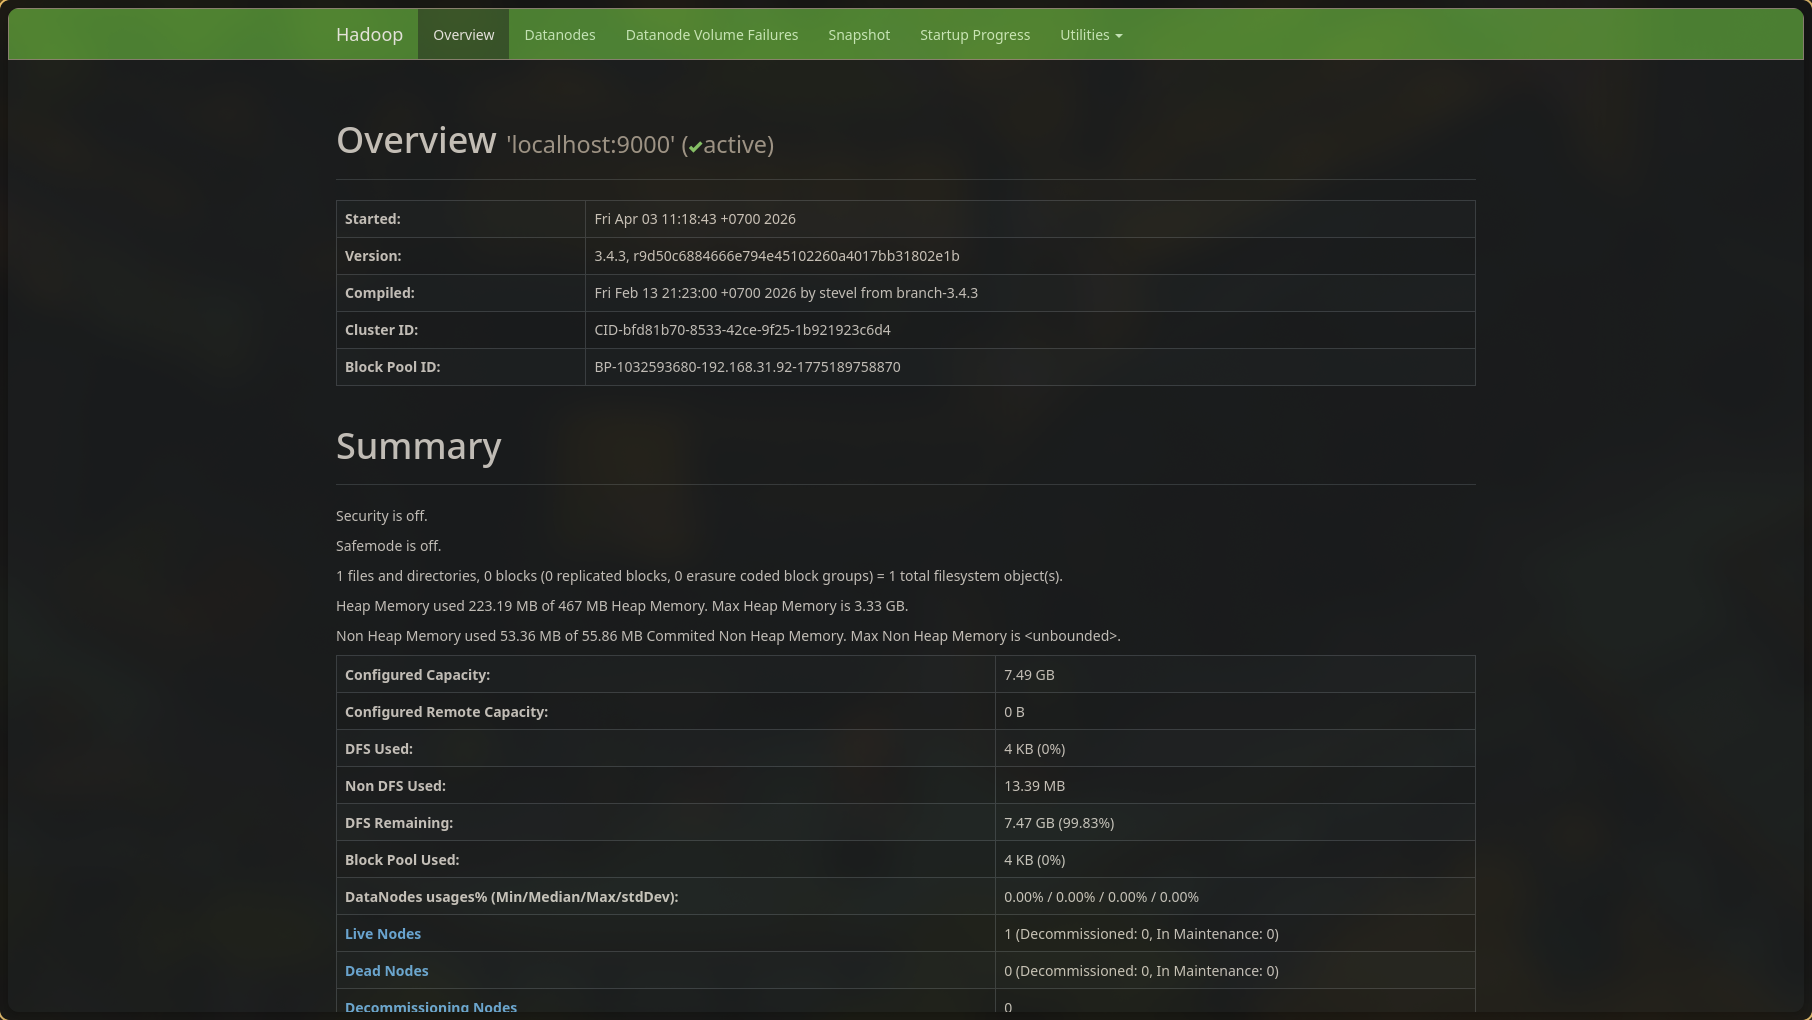
\includegraphics[width=0.9\textwidth]{images/pseudo-8.png}
    \caption{Giao diện giám sát HDFS NameNode.}
    \label{fig:pseudo-namenode-ui}
\end{figure}

\begin{figure}[H]
    \centering
    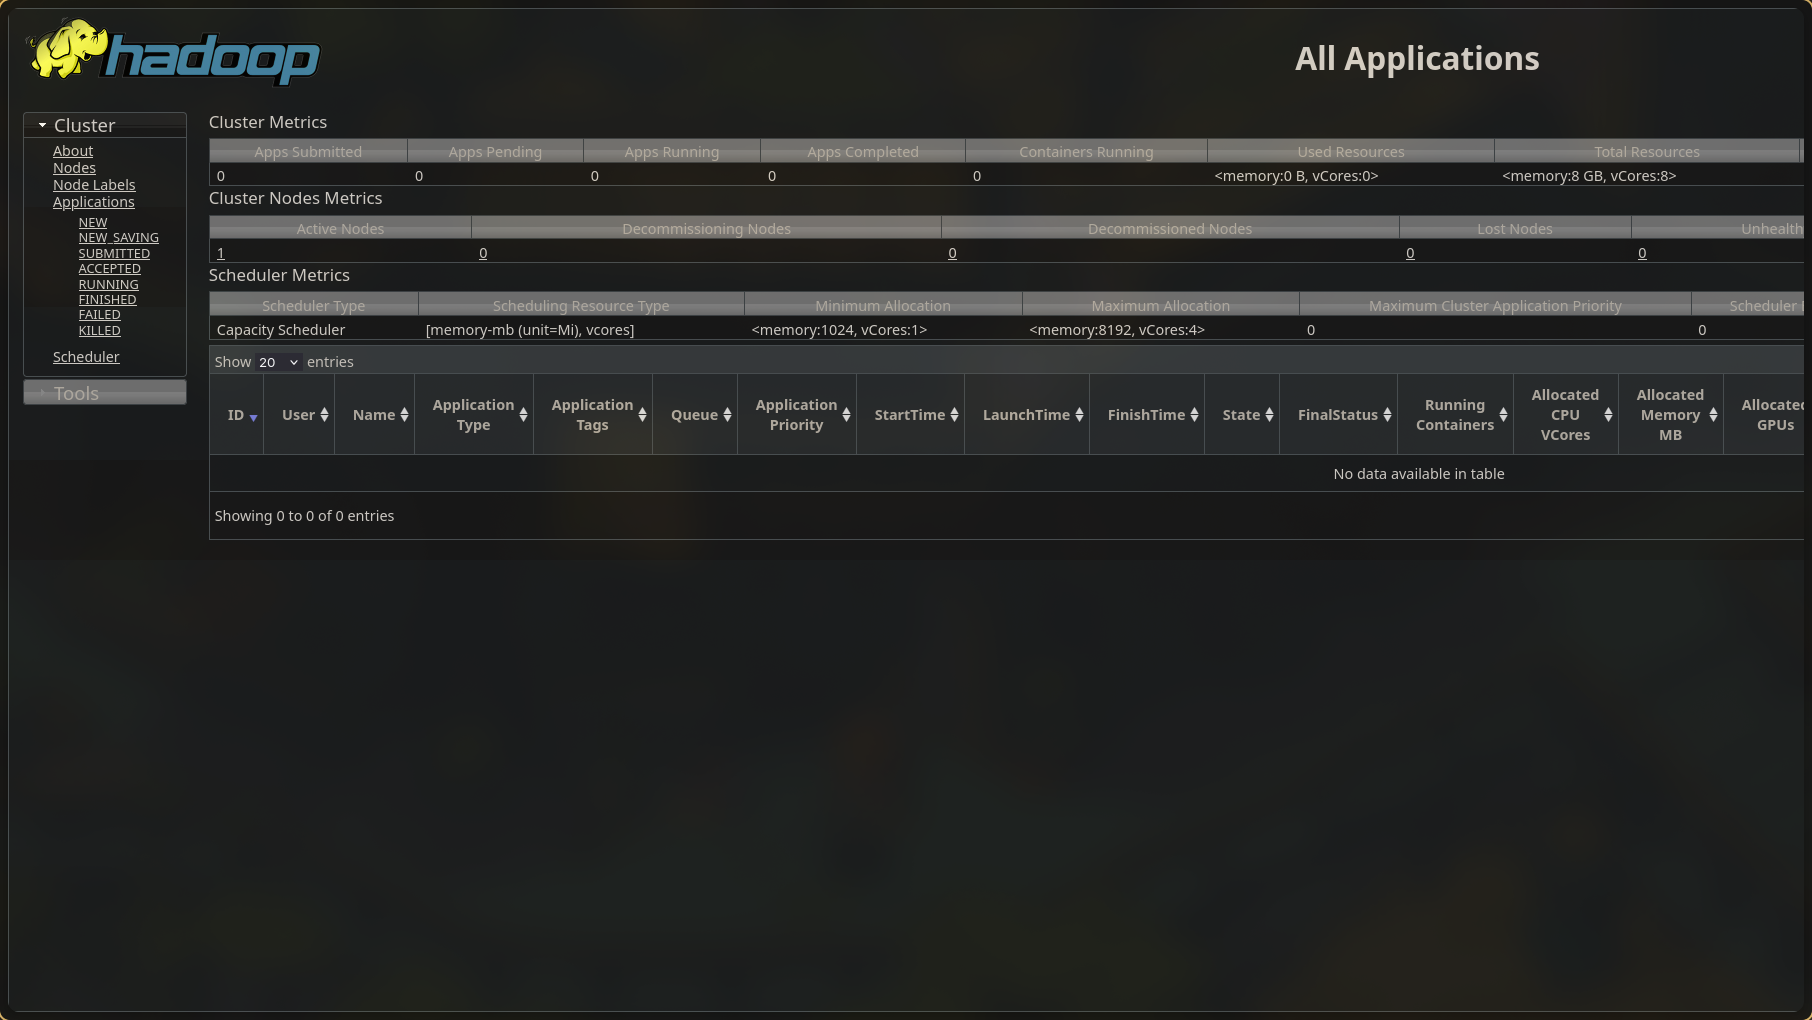
\includegraphics[width=0.9\textwidth]{images/pseudo-9.png}
    \caption{Giao diện giám sát YARN ResourceManager.}
    \label{fig:pseudo-yarn-ui}
\end{figure}

\subsection{Xử lý sự cố}

Phần này ghi nhận các lỗi gặp phải trong quá trình cài đặt, phương pháp tra cứu và cách khắc phục.

\subsubsection{Lỗi \texttt{hostname: command not found}}

\textbf{Mô tả lỗi:} Khi thực thi lệnh \texttt{start-dfs.sh}, hệ thống báo lỗi \texttt{line 129: hostname: command not found}. Nguyên nhân do lệnh \texttt{hostname} không được cài đặt mặc định trên Arch Linux.

\textbf{Cách khắc phục:} Cài gói \texttt{inetutils} cung cấp lệnh \texttt{hostname}:

\begin{lstlisting}[language=bash, numbers=none]
sudo pacman -S inetutils
\end{lstlisting}

Sau khi cài đặt, lệnh \texttt{hostname} hoạt động bình thường và \texttt{start-dfs.sh} chạy lại mà không còn cảnh báo:

\begin{figure}[H]
    \centering
    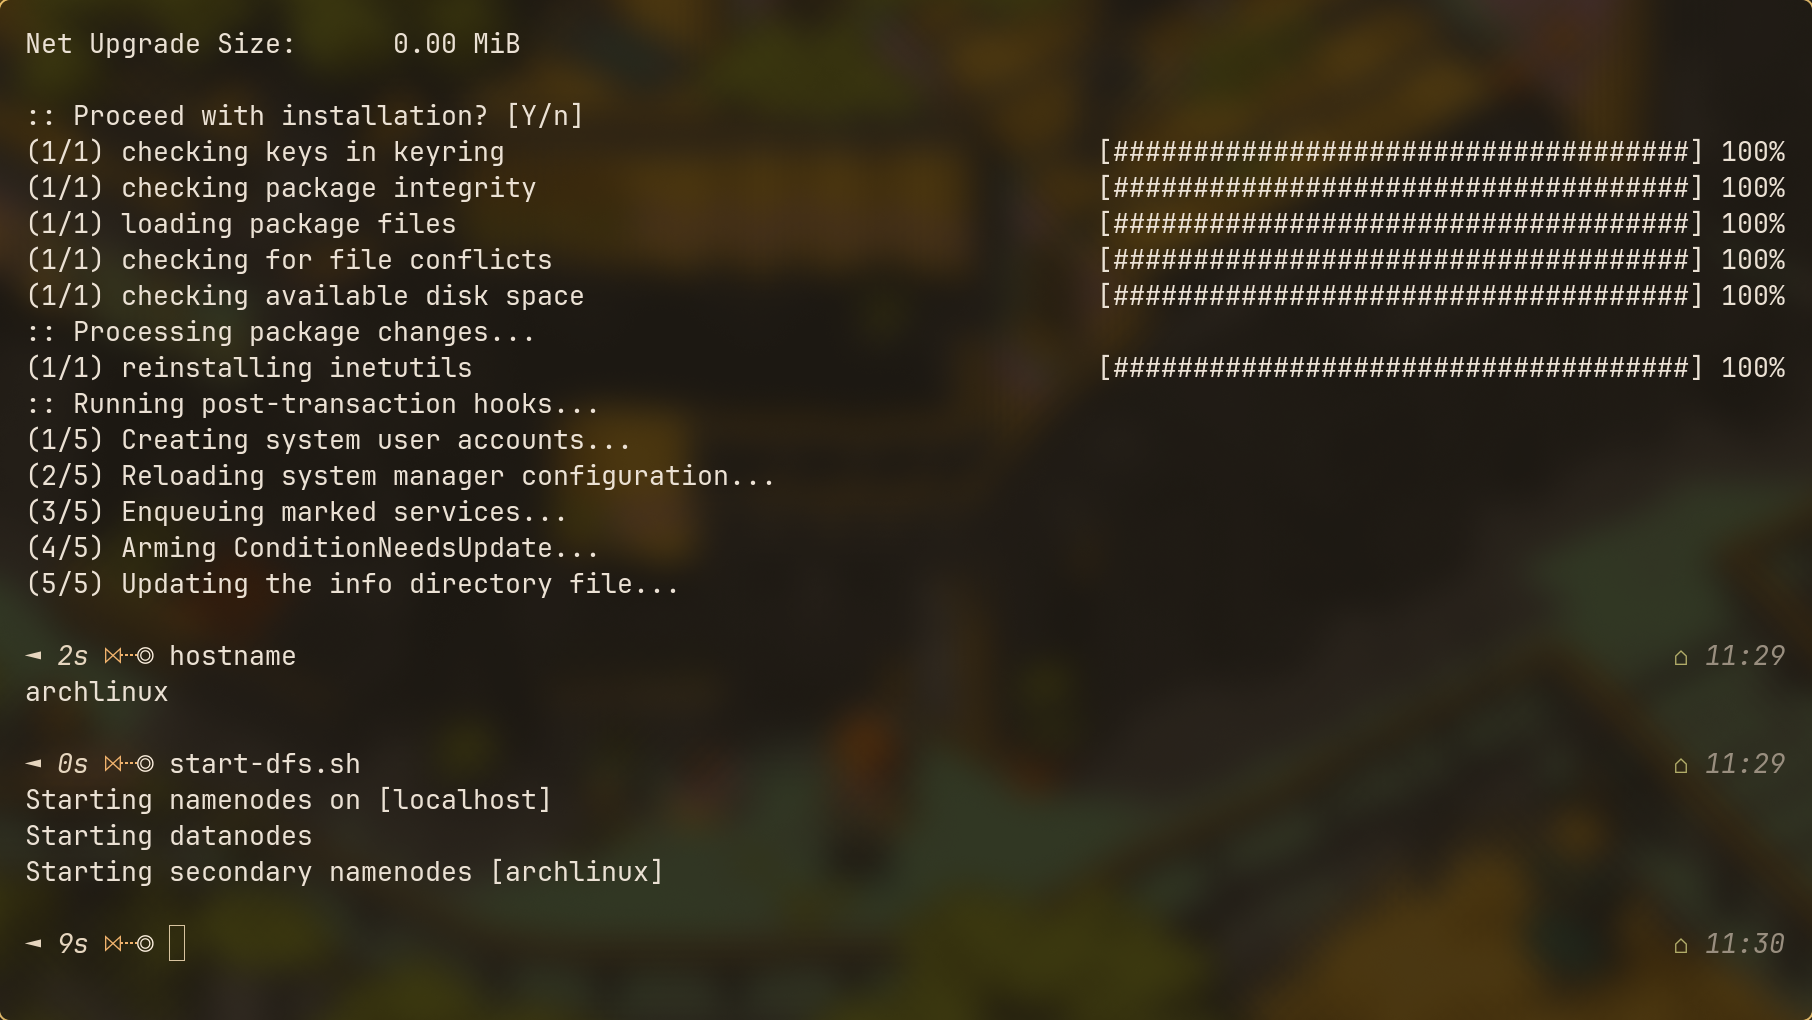
\includegraphics[width=0.8\textwidth]{images/pseudo-10.png}
    \caption{Sau khi cài \texttt{inetutils}: \texttt{start-dfs.sh} chạy thành công không còn cảnh báo \texttt{hostname}.}
    \label{fig:pseudo-hostname-fix}
\end{figure}
